
\section{density.xml}

The density file contains density constraints for the RBA model.


\subsection{RBADensity}
\label{sec:rba_density}

The outermost portion of the density file is an instance of class
\rbadensity, shown in Figure~\ref{fig:density_doc}.

\begin{figure}
  \centering
  \includegraphics[scale=0.8]{figures/density_doc}
  \caption{XML structure of density document.}
\label{fig:density_doc}
\end{figure}

\rbadensity{} has no simple attributes.
It includes exactly one instance of \textbf{ListOf} container classes.
All \textbf{ListOf} classes do not have own attributes,
they are merely used to organize a list of instances from another class.

\subsection{TargetDensity}
\label{sec:target_density}

The \targetdensity{} class is used to define density constraints
(Fig.~\ref{fig:density_doc}).
In a RBA model, a density constraint defines how many molecules
a given compartment can contain.
It inherits \targetvalue{} for the constraint definition part.

\paragraph{The \textit{compartment} attribute}
The \textbf{compartment} attribute must match the identifier of a \compartment.


\subsection{TargetValue}
\label{sec:target_value}

The \targetvalue{} class is used to define the sign of an additional RBA
constraint and the value of its second member
(Fig.~\ref{fig:density_doc}).
It is designed to be inherited.
The child class usually holds information about the first member of the
constraint
(\textit{e.g.} compartment for a density constraint,
metabolite for a production constraint).

\paragraph{The \textit{value}, \textit{lb} and \textit{ub} attributes}
Every attribute can be left undefined, or
contain the identifier of a \function{} or an \aggregate.

If \textbf{value} is defined, the constraint is an equally constraint.
\textbf{lb} and \textbf{ub} are ignored.
If \textbf{value} is undefined, \textbf{lb} (resp. \textbf{ub}) defines
a lower bound (resp.\ upper bound) inequality constraint.
Note that \textbf{lb} and \textbf{ub} may both be defined, yielding two
separate inequality constraints.
